\documentclass{report}
\usepackage{graphicx} % Required for inserting images

\usepackage[sorting=none]{biblatex}
\addbibresource{refs.bib}

\usepackage{float}
\usepackage{changepage}
\usepackage[hidelinks]{hyperref}
\usepackage{parskip}
\usepackage{XCharter}
\usepackage[T1]{fontenc}
\usepackage{amsmath}
\usepackage{amssymb}
\usepackage{glossaries}
\usepackage{pgfgantt}

\usepackage[a4paper,margin=1in]{geometry}

\linespread{1.2}
\emergencystretch 3em

\renewcommand{\labelenumii}{\arabic{enumi}.\arabic{enumii}}

\makeglossaries

\newglossaryentry{llvm}
{
    name=LLVM,
    description={A compiler backend software that optimises and IR and converts it to an executable program}
}

\newglossaryentry{ir}
{
    name=IR,
    description={An intermediate representation, a version of the program code that has been converted to a simpler form making it easier to optimise}
}

% \newglossaryentry{llvmir}
% {
%     name=LLVM IR,
%     description={The intermediate representation used by LLVM}
% }

% \newglossaryentry{cpu}
% {
%     name=CPU,
%     description={Central Processing Unit}
% }

\newglossaryentry{ast}
{
    name=AST,
    description={Abstract Syntax Tree}
}
\newglossaryentry{octree}
{
    name=Octree,
    description={A data structure where each internal node has 8 children. Typically used to store points (e.g. particles) in a 3D space for faster search algorithms}
}

\newglossaryentry{dsl}
{
    name=DSL,
    description={Domain Specific Language}
}

\newglossaryentry{sph}
{
    name=SPH,
    description={Smoothed Particle Hydrodynamics}
}

\newglossaryentry{mpi}
{
    name=MPI,
    description={Message Passing Interface, a tool for multi-node parallel computation}
}

\newglossaryentry{openmp}
{
    name=OpenMP,
    description={Open Multi Processing, a tool for parallelising programs across multiple processing cores}
}

\newglossaryentry{cuda}
{
    name=CUDA,
    description={Compute Unified Device Architecture, an API allows software to use Nvidia GPUs for general purpose processing}
}



\begin{document}

\newcommand\ProjectTitle{Accelerating Performance of SPH Simulations\\ Using DSL Methods with Exascale Techniques}
\newcommand\Title{Project Specification}
\newcommand\Author{D\'eveloppement Sans Logique}
\newcommand\Department{Department of Computer Science}
\newcommand\Institution{University of Warwick}
\newcommand\YearOfStudy{Year of study: 2023/2024}
\newcommand\Supervisor{Supervisor: Dr Gihan Mudalige} % TODO: Dr or Prof
\newcommand\Team{Tom White, Scott Parker, Maciej Waszczuk,\\ Miko\l{}aj W\k{a}sacz, James Macer-Wright, Tom Divers}

\begin{titlepage}
    \begin{center}
        \vspace*{1cm}

        \huge\textbf\Title \\
        \vspace{1cm}
        \Large\textbf\ProjectTitle

        \vspace{1cm}

        \large\textbf\Author \\
        \textit\Team \\

        \vspace{1cm}
        
        \Department \\
        \Institution

        \vfill

        \Supervisor \\
        \YearOfStudy

        \vspace*{3cm}
        % \vfill
        
        \begin{adjustwidth}{-1in}{-1in}
            
\includegraphics[width=\paperwidth]{thesis/graphics/line.png}
        \end{adjustwidth}
    
        \vspace*{-1.0cm}
        
    \end{center}
\end{titlepage}


\tableofcontents

\printglossary [nonumberlist]

% TODO: Basic Overview of the project architecture ?

% TODO
\chapter{Introduction}

Smooth Particle Hydrodynamics (SPH) is a mesh-free Lagrangian method used to obtain approximate solutions to fluid dynamics problems by simulating a large number of particles and their interactions \cite{liu2010smoothed}. This has been used extensively in scientific and industrial applications. These applications include simulations of dam breaking \cite{monaghan1994simulating} and rigid bodies such as a ship hull impacting water \cite{veen2010smoothed}. SPH can also be easily extended to other problems such as gases or dust fluids \cite{monaghan1995sph}, and thermal and matter diffusion. It is extensively used in the special effects and graphics industry, including video games, movies and TV advertising \cite{monaghan2005sph}.

Due to the practical nature of the SPH problem, many software frameworks and libraries have been developed. In order to obtain meaningful results from SPH simulations, a very large number of particles must be considered. Additionally, the equations describing the particles' behaviour are fairly complex. Hence, large-scale simulations require massive amounts of computing power, far beyond the capabilities of a typical desktop PC. Because of this, high-performance computing nodes or clusters are used to perform such simulations. Such systems are characterised by high levels of parallelism, which requires the simulation code to be written in a way that can fully utilise these parallel systems.

Writing programs for high-performance systems is complex, as it requires in-depth knowledge of the target system in order to fully exploit its performance. This results in high-performance programs being expensive to develop and difficult to maintain. To address this issue, many libraries have been developed that aim to facilitate this process. Such libraries are often specific to a specialised problem domain and target platform. One of the techniques to making the code more readable and easier to write is using a Domain-Specific Language (DSL). 

A DSL is a specialised programming language that includes convenient syntax for describing common operations in a specific problem domain. Since SPH simulations typically have similar structure and use a common class of operations, they are well-suited to be described using a specially-designed DSL. This is why we decided to use this technique to develop a framework that aids in creating SPH programs. This approach has another benefit of enabling the user to write platform-independent code, since the framework handles parallelism and applies problem and architecture specific optimisation techniques.


% TODO
\chapter{Background}

\section{Domain Selection}
Selecting an appropriate domain for a DSL project is important, as there is a balance to strike between how populated with research the areas are.

A domain with a large amount of research (e.g. Monte Carlo simulations) is likely to have a large amount of well-documented optimisations, with many example miniapps to look at to find common code between. This makes it easier to know what the generated code must look like. However, DSLs may already exist for the domain, resulting in the project not contributing greatly to the field of research.

A domain with very little research (such as Multi-material) is the opposite. It is difficult to find generalising optimisations that can be applied in the area without being an expert in that domain's specific computations, and very familiar with any fresh research surrounding it. There may also not be many, if any at all, miniapps that demonstrate the techniques used in the domain. Additionally, there may not be a widely agreed-upon architecture for the representation of the data structures for the domain.

This meant a number of possible domains were considered by the team and supervisor to ensure the project is well-realised, thought-out and that issues stemming from the domain selection do not come up later, hindering the scope of the project or costing significant development time.

The alternative domains that were considered, are described below, and reasons are given as to why the final chosen domain was favoured over them.


\subsection{Monte Carlo}\label{sec-montecarlo}
Monte Carlo simulations make use of statistical models to estimate mathematical functions and model complex systems. In a Monte Carlo Simulation, a system is modelled as a series of probability density functions (PDFs), the PDFs are repeatedly sampled from, and the results have some aggregate function applied to them to generate a statistic \cite{harrison2010introduction}.

Monte Carlo problems are highly parallelisable, as there is no communication between threads until the aggregate function is performed at the end of computation. This makes them highly applicable to high performance computing, where they can be distributed across GPUs and compute nodes at a high scale.

However, due to the simplicity of this problem, there are many existing DSLs that have examined the Monte Carlo problem. These include Neb \cite{lindsey2016domain} which generates C++ code targeting GPUs and FPGAs from equations written in LaTeX, and Contessa \cite{thomas2007domain} which generates code targeting FPGAs from a functional subset of C.

As a result, we decided that designing a DSL for a problem domain with a less saturated research field would be a more relevant project, and result in a greater contribution to the DSL space.

\subsection{Multi-material}\label{sec-multimaterial}
In many scenarios it would be useful to simulate involve more than a single material. This form of simulation is particularly challenging, with no standard procedure or best solutions agreed on in the little available literature, given this is a relatively new field. 

This was considered as a potential direction for the project, though it was concluded that a more populated area is more feasible for this project. This project would be hard to find performance comparisons for due to a lack of available miniapps. Another consequence of this is that it would be far beyond the scope to find our own optimisations or create our own efficient code with no frame of reference.

\section{Smooth Particle Hydrodynamics}

SPH simulations (discussed extensively in \cite{monaghan2005sph}) are typically used to simulate the mechanics of a continuous medium. This is done by discretising the medium into a collection of Lagrangian particles. In order to simulate some field $f: \Omega \rightarrow \mathbb{R}$ over a domain $\Omega \subseteq \mathbb{R}^d$, we find the following for each particle $i$ located at $\textbf{r}_i \in \mathbb{R}^d$:

\begin{equation} \label{eq:sph_integral_equation}
    f(\textbf{r}_i) = \int_{\Omega} f(\textbf{r}) W( \textbf{r}_i - \textbf{r}, h) d\textbf{r} 
\end{equation}
$W(\textbf{r}_i - \textbf{r}, h)$ is referred to as a \textit{kernel function}, and governs how the values of $f(\textbf{r})$ around $\textbf{r}_i$ affect $f_i$. We assume that $W$ is radially symmetric with respect to $\textbf{r}_i$. $h \in \mathbb{R}$ is referred to as the \textit{smoothing radius}, and allows us to adjust the shape of the kernel. A one-dimensional example of such a kernel is the Gaussian kernel, given by

\begin{equation}
    W(x, h) = \frac{e^{-x^2 / h^2}}{h \sqrt{\pi}}
\end{equation}

\newcommand{\norm}[1]{\left\lVert#1\right\rVert}

We assume that the mass of each particle $m_i$ is constant throughout the simulation; therefore, each of the particles has volume $V_i = m_i / \rho(\textbf{r}_i)$, where $\rho : \Omega \rightarrow \mathbb{R}$ is the density of our medium. Therefore, in order to compute equation \eqref{eq:sph_integral_equation}, we approximate it by summing over $N(i) := \{j : \norm{\textbf{r}_j - \textbf{r}_i}_2 \leq \epsilon\}$, the set of all particles at most $\epsilon$ away from $i$ \cite{zhang2021sphinxsys}:
\begin{equation} \label{eq:particleSummation}
    f(\textbf{r}_i) \approx \sum_{j \in N(i)} V_j  \cdot W(\textbf{r}_i - \textbf{r}_j, h) \cdot f(\textbf{r}_j) = \sum_{j \in N(i)} \frac{m_j}{\rho_i} \cdot W(\textbf{r}_i - \textbf{r}_j, h) \cdot f(\textbf{r}_j)
\end{equation}
Note that $\rho(\cdot)$ is also a field over $\mathbb{R}^d$; therefore, we can also compute it using equation \eqref{eq:particleSummation}:
\begin{equation}
    \rho(\textbf{r}_i) \approx \sum_{j \in N(i)} \frac{m_j}{\rho(\textbf{r}_j)} \cdot W(\textbf{r}_i - \textbf{r}_j, h) \cdot \rho(\textbf{r}_j) = \sum_{j \in N(i)} m_j \cdot W(\textbf{r}_i - \textbf{r}_j, h)
\end{equation}

We can use this particle summation method to compute the gradient of $f$ as
\begin{align}
\begin{split}
    \nabla f(\textbf{r}_i) &= \int_{\Omega} \nabla f(\textbf{r}) W(\textbf{r}_i - \textbf{r}, h) dV = - \int_{\Omega} f(\textbf{r}) \cdot \nabla W(\textbf{r}_i - \textbf{r}, h) dV\\
    &\approx - \sum_{j \in N(i)} V_j \cdot \nabla_i W_{ij} \cdot f(\textbf{r}_j)
\end{split}
\end{align}
where $\nabla_i W_{ij} := \nabla_{\textbf{r}_i} W(\textbf{r}_i - \textbf{r}_j, h)$ is the gradient of our smoothing function in the direction of $\textbf{r}_i$. Similar derivations can be used to compute other derivatives of $f$. 

Considering we have not specified the field we are trying to simulate, the framework above remains very general. Consequently, this framework can be used to simulate a wide variety of phenomena, in areas ranging from fluid dynamics to astrophysics \cite{monaghan2005sph}. 

%Here, we will discuss how this framework can be used to simulate fluid flow according to the Navier-Stokes equations.

%Fluid 

Computing these particle-average sums gives rise to several challenging computational problems. One such problem stems from the fact that this framework is meshless. Because of this, computing $N(i)$ efficiently is a challenging and computationally expensive problem with a wide variety of existing algorithms \cite{dequn2012nnsearch, prabhu2021pysph, fernandez2022octree}. This is especially true in a multi-node setting, where data locality is vital \cite{sphexa, keller2023cornerstone}. We aim to simplify, abstract and partially automate the implementation of efficient and parallel algorithms for this task with our DSL. 

\section{Prior Work}
SPH simulations have been an active research area ever since their introduction; consequently, prior efforts to coalesce their features into libraries and domain-specific languages. However, we believe that an active-library DSL (in a similar vein to OPS \cite{reguly2014ops} and OP2 \cite{mudalige2012op2}) will fill a gap by providing new functionality and flexibility compared to existing solutions. It is also important to be familiar with features present in other related projects as to offer a viable product at the end, without missing features that experts in the field may find obvious and essential.

\subsection{OPS \cite{reguly2014ops} \& OP2 \cite{mudalige2012op2}}

OPS and OP2 are DSLs developed for specific problem domains that compile code written with their API to many different hardware platforms. This results in performance portability, near-optimal performance, and scaling on modern multi-core and many-core processor based systems. OPS targets algorithms over a structured mesh, which has a fixed topology of meshes, and OP2 targets algorithms over an unstructured mesh, which stores connectivity information to specify the mesh topology.

OP2 generates the target code by using Clang to generate an AST of the program, extracting key values from the kernel functions using this AST. These are then transformed as necessary, then used to populate templates of the target code developed for each backend.

A program in these DSLs is implemented via an access-execute pattern, where the user

\begin{enumerate}
    \item Initialises the state of the data structure with OPS/OP2, by manually setting values or importing larger datasets with HDF5

    \item Writes kernel functions for iterations and reductions

    \item Declares the kernel functions with OPS/OP2 and specifying their data access patterns and other information about the functions
\end{enumerate}

The DSL we develop will take heavy inspiration from the library design and architecture of OPS/OP2.

\subsection{SPHinXsys \cite{zhang2021sphinxsys}}

SPHinXsys is an open-source library designed to simplify the process of writing SPH systems. It supports simulations of a large variety of physical objects and phenomena, including Newtonian and non-Newtonian fluids, rigid and elastic solids, diffusion-reaction processes, amongst others.\footnote{SPHinXsys's official documentation can be found at \href{https://www.sphinxsys.org/}{\texttt{www.sphinxsys.org}}.} It is unlikely that we will be able to develop a DSL that accommodates all of these features in such a short amount of time; however, we do expect to be able to develop a solution that has several advantages over SPHinXsys.

One of these advantages comes in the form of optimisations. By choosing to implement a DSL instead of a traditional library, we expect to be able to apply several optimisations to input programs \textit{before} compile-time. Such optimisations are not possible for traditional libraries, and SPHinXsys does not make use of them.

To run simulations in parallel, SPHinXsys uses Intel's TBB C++ template library as a backend. In our DSL, we intend to include support for a variety of different backends, including OpenMP, CUDA and MPI (which is made significantly easier by choosing to write a DSL), thus allowing for a wider array of system architectures.

\subsection{PySPH \cite{prabhu2021pysph}}

PySPH is an extensive Python framework for writing SPH simulations that targets OpenMP, MPI and CUDA. Architecturally, this library is very similar to the DSL that we intend to implement.

PySPH promises a lot of flexibility in the algorithms it uses, and allows the user to switch out some part of a simulation's implementation in a very modular way. PySPH claims performance to be ``comparable to handwritten solvers implemented in FORTRAN'', but their performance report within the main published paper claims to be around 50\% slower than DualSPHysics v5.0, a handwritten C++ SPH solver. This is due to DualSPHysics' more rigid design, as it ``does not allow us to replace the NNPS algorithm easily''. It is mentioned that there is still a lot of performance to get out of the framework, though it is practically impossible to reach parity given the nature of Python, and the reliance on Cython's compiler to be optimal.

By using C++ we hope to get better performance compared to PySPH, while maintaining its flexibility of being able to implement a wide range of SPH problems.

%TODO: Can reintroduce these sections, commented out for now
\subsection{Nauticle \cite{havasitoth2020nauticle}}
Nauticle is a YAML-based DSL for particle-based simulations. It allows users to specify a system of equations, and then uses the Arboria library to simulate them \cite{robinson2017arboria}.

Nauticle has the advantage of being relatively easy for users without programming experience to learn. In order to accommodate for this, however, Nauticle sacrifices flexibility. It is also relatively limited in terms of performance and target architectures, and does not provide parallel implementations for OpenMP, CUDA, or MPI (we intend to target all three with our solution). 



% Include explanation of what a miniapp is, which exist in the SPH space

\section{Miniapps}

A reduced, proxy application or miniapp encapsulates the performance-intensive component of many scientific or research based workloads in a simpler version of the application \cite{miniapps}. This results in a more easily understandable and modifiable codebase that still represents the main performance characteristics of the workload. Existing miniapps implementing the SPH problem were investigated as part of the research for this project, to gain a greater understanding of the SPH algorithms and how they can be accelerated. This includes SPH-EXA \cite{sphexa}, a miniapp targeting exascale computation with backend implementations using 
%Have references for these or have a glossary 
MPI, OpenMP and CUDA, as well as PBF-SPH \cite{pbfsph}, a simpler SPH miniapp with backends using OpenMP, OpenCL and SYCL.

\subsection{SPH-EXA}
SPH-EXA is a miniapp written by the HPC Group at the University of Basel, it is a SPH simulation written for C++20 which supports a number of different technologies. Specifically, MPI, OpenMP, CUDA and HIP. The motivation behind the miniapp was to ``extrapolate common basic features of SPH simulations and consolidate them in a fully optimised, Exascale-ready package'' \cite{sphexa}.

The package implements a number of well known test simulations, such as ``sedov'' (spherical blast wave) and ``evrard'' (spherical collapse) \cite{sedov, evrard, sphtests}. It also supports the use of custom initialisation files for these scenarios, or alternately simply specifying the side lengths of a cube of particles in the simulation. When running the simulation, the developer can control the number of iterations or give a real length of time for the simulation. Similarly, it supports outputting a dump of particle data and various properties at a controllable number of iterations (e.g. particle position, velocity, density). This data is aggregated in a HDF5 file, which provides a compact structured data storage format which is effective both in serial and parallel \cite{hdf5}.

Similarly, SPH-EXA supports both running serially or in MPI, both with OpenMP controlling parallelism in each node. It also builds an executable for running the simulation on GPUs using CUDA. Experience testing the miniapp reveals issues with the parallel HDF5 writing, with severe I/O bottlenecks on iterations which dump particle data out to file. % TODO: more 

SPH-EXA uses an octree internally as part of a specialised custom library called ``Cornerstone'' to distribute particle between nodes, as well to provide a data structure to efficiently represent the 3-dimensional simulation space at a low level and provide an efficient way to do nearest neighbour operations in the iteration. From the sequencing diagram of the iteration process included in the documentation finding nearest neighbour particles takes $\sim$10\% of the total iteration time, and this is a critical operation to perform efficiently, especially distributed over multiple nodes, to keep the program performance high. We will consider using a similar octree-based model in our project. 



% TODO
\chapter{Objectives} % Function and Non-Functional requirements

In order to ensure our system fulfils its intended purpose, we have devised a formal list of requirements. This will allow us to track progress and measure the success of the project. The requirements have been categorised and prioritised, according to the MoSCoW method. In particular, ``must'' means that a requirement is essential for the project and will be considered first. ``Should'' denotes the requirements that are important but not strictly necessary. ``Could'' means that a requirement is of less importance and will be implemented provided that the time constraints allow it. We have also identified the objectives which are out of scope for this project, and therefore will not be implemented. Such objectives are labelled as ``won't''.

\section{Objective List}
% Feel free to add/change anything
\begin{enumerate}
    \item Problem domain
    \begin{enumerate}
        \item The system \textbf{must} facilitate writing code for common SPH problems.
        \item The system \textbf{won't} support other problems outside of the SPH domain, such as gravitational interaction or Discrete Vortex Method (DVM).
    \end{enumerate}
    \item Input code
    \begin{enumerate}
        \item The system \textbf{must} handle input code written in C++, potentially with some syntax extensions.
        \item The system \textbf{should} use existing C++ syntax whenever possible.
        \item The system \textbf{could} process written equations into kernel functions for the user.
        \item The system \textbf{won't} process input code written in other languages, such as Python.
    \end{enumerate}
    \item API design
    \begin{enumerate}
        \item The system \textbf{must} expose a low-level API, similar to OPS and OP2.
        \item The system \textbf{should} allow the user to implement some functions in a platform-specific way (e.g. if they want to integrate an existing SPH HPC library).
        \item The system \textbf{could} implement a high-level API, to further simplify developing SPH simulations (e.g. use operator overloading to allow the user to define parts of the program as equations).
    \end{enumerate}
    \item Target platforms
    \begin{enumerate}
        \item The system \textbf{should} support multiple target processor architectures.
        \item The system \textbf{should} be able to generate code for OpenMP.
        \item The system \textbf{should} be able to generate code for CUDA.
        \item The system \textbf{could} be able to generate code for MPI.
        \item The system \textbf{could} implement combinations of platforms, such as CUDA + OpenMP or CUDA + MPI.
    \end{enumerate}
    \item Performance
    \begin{enumerate}
        \item The system \textbf{should} generate code that achieves performance no more than 10\% slower than the reference miniapp implementations.
        \item The system \textbf{could} implement more advanced optimisations to further improve performance.
        \item The system \textbf{should} be able to compile input code in reasonable time.
    \end{enumerate}
\end{enumerate}

\section{System Overview}

Figure \ref{fig:arch-diagram} gives a broad overview of the proposed project architecture to meet the above objectives. Broadly, we take the C++ code written with our DSL, and parse it. Extract the AST and then generate suitable code for one of a number (or a combination) of backend hardware using a template engine. In the process, applying transformations or optimisations as necessary. This is then compiled by the usual C++ toolchain, which can apply further compiler optimisations. Optionally, if time permits, we want to also develop a separate parser which can take a more elementary equation based representation of the SPH simulation and convert that into a representation based in our DSL.

\begin{figure}[H]
    \centering
    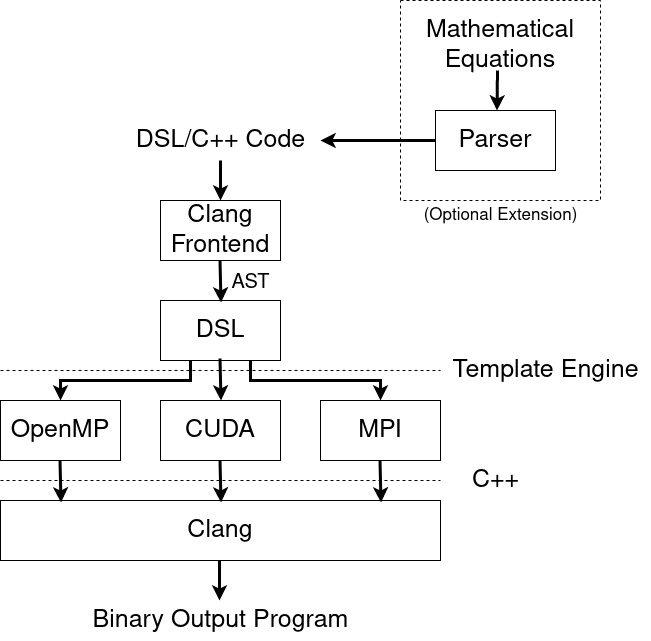
\includegraphics[width=0.8\textwidth]{thesis/diagrams/architecture.jpg}
    \caption{Overview of the proposed project architecture.}
    \label{fig:arch-diagram}
\end{figure}

% TODO: proofing
\chapter{Resources}

Throughout the development of the project, we anticipate requiring several open source technologies and projects. These will vastly aid development, by saving time re-implementing common functions such as hardware compatibility or control, or by providing comparisons of performance and results for testing efficiency or validating program correctness. Furthermore, high-end multi-node multi-core computing systems are prohibitively expensive, so for practical purposes it is more feasible to utilise these systems. 

% Stuff which will be used to test the DSL against
\section{Miniapps}

Miniapp (or ``Mini-App'') is a miniature application which captures the inherent computational complexity of the problem domain whilst still keeping a small enough codebase to be manually analysed (or optimised). The term was coined fairly recently, and while there is no concrete definition of what a miniapp \textit{is}, they also resemble closely benchmark applications developed previously \cite{miniapp}.

We are planning on using two miniapps (SPH-EXA \cite{sphexa} and PBF-SPH \cite{pbfsph}), which both implement SPH simulations for a number of different test scenarios, each targeting a number of different backends. 

The use of miniapps in this project will be twofold: Firstly, as a benchmark. The miniapps are hand optimised to run on specific backend technologies such as PBH-SPH which runs on OpenMP, MPI, CUDA, OpenCL and SYCL. By comparing the run time of programs automatically generated by the project to these hand optimised programs we can get a benchmark of how much overhead our project adds to the expected performance a user would expect.

Secondly, we can use the miniapps to provide a simple verification check that the project is outputting the expected solutions to the simulation. The SPH-EXA miniapp includes a number of test simulations such as ``sedov'' \cite{sedov} (spherical blast wave), ``noh'' (spherical implosion), ``evrard'' (gravitational collapse of an isothermal cloud), ``turbulence'' (turbulence in a box) and ``kelvin-helmholtz'' (Kelvin-Helmholtz instability in a slice). This will be in addition to other measures taken to ensure program verification and validation detailed in the testing chapter.

% OpenMP, MPI, CUDA, OpenCL, etc?
\section{Libraries}

As previously mentioned, the intention of this project is to develop a portable language which supports a number of high performance computing backends. These are often specialised or dedicated hardware architectures which require custom compiler wrappers or even open source libraries to provide compatibility to a higher level C++ API. 

The backends we aspire to be able to support are the following. Note that due to time constraints, we may have to prioritise the initial and more common backends.  
\begin{itemize}
    \item \textbf{Serial} - Technically this is the absence of a specialised backend. However, it is important to note that the programs should be capable of being run in a serial environment. Perhaps taking advantage of other CPU optimisations such as SIMD vectorisation (i.e. AVX) though Intel Intrinsics library \cite{intrinsics}.
    \item \textbf{OpenMP} - This is the main library which supports shared memory parallel programing on CPUs in C++. It is intended that this be a primary focus for the project \cite{openmp}.
    \item \textbf{MPI} - Message Passing Interface is a standardised paradigm for multi-node parallel computing architectures. This involves orchestrating multiple independent CPUs through message passing. MPI is commonly implemented through an open source library, and we are planning on using OpenMPI \cite{openmpi}.
    \item \textbf{CUDA} - CUDA is the primary parallel computing model developed by Nvidia for GPUs. CUDA is available in C++ through the Nvidia provided library and nvcc compiler \cite{nvcc}.
    \item \textbf{SYCL \& OpenCL} - A group of related technologies which are an open source alternative for developing parallel compute programs on GPUs \cite{sycl}. 
    
    % TODO: more on this?
    % TODO: any more backends?
\end{itemize}

In addition to the above general purpose libraries, the project is planned to involve a code generation functionality to create the optimised code for each backend. One method to implement this from a high level standpoint is to use Jinja \cite{jinja} templates. These are short code snippets defined in a high level templating language called Jinja which are then placed in source code files before being compiled. Another option is to instead use the LLVM \cite{llvm} parser and then directly manipulate the generated abstract syntax tree of the program. 

Furthermore, the nature of particle simulations is that there will be a large amount of data to be dumped out from running simulations for visualisation or debugging purposes. One way of managing this in a parallel computing friendly way, as well as keeping file sizes small, is using a format such as HDF5 \cite{hdf5}, which provides a structured and compact storage medium for the data. In addition, the Silo \cite{silo} library from LLNL\footnote{Lawrence Livermore National Laboratory} allows the stored data to be easily read by other programs, such as Python for analysis, or open source visualisation platforms like VisIt \cite{visit}.

% DCS Batch compute? etc?
\section{Hardware}

To take advantage of the full potential of the massively parallel architectures we plan to use we will require the use of a much more powerful computing system than is available in personal computing hardware. We therefore plan to make use of two systems available at the University of Warwick:

\begin{itemize}
    \item \textbf{DCS Batch Compute} - The Department of Computer Science's batch compute system allows for both CPU and GPU tests involving both single node and multi-node programs. The CPU partitions utilise Intel Xeon E5-2660 v3 with 5 nodes / 200 threads available, while the GPU partitions utilise Nvidia A10s. \\ 
    This system is also particularly useful for consistent benchmarking as they have fewer background processes running on them compared to traditional machines.
    \item \textbf{Scientific Computing RTP} - The University also provides access to more powerful compute clusters which are part of HPC Midlands \cite{scrtp}.
\end{itemize}

% GitHub, overleaf and stuff the project will need to aid development
\section{Software}

In addition to the specialised hardware and libraries used to develop the project, we plan to use other software services to support project development.
\begin{itemize}
    \item \textbf{GitHub} - The university provides an enterprise GitHub solution, which will be useful for version control and managing contributions between a large team working on multiple parts of the project simultaneously. It will also support the project management portion with GitHub Projects, providing a simple Kanban board implementation to keep track of important tasks and pending deadlines. Furthermore, GitHub Actions will allow automated testing to be run regularly to ensure correctness. 
    
    \item \textbf{Visual Studio Code} - A lightweight IDE which supports C++ development as well as git version control. In addition, the remote functionality will enable development on target architecture as well. 
   
    \item \textbf{Slurm} - A job scheduler used by the department to schedule jobs on the specific hardware. It will also allow deploying tasks and monitoring their status automatically via email, instead of having to stay at terminals continually during runtime. 

    \item \textbf{GTest} \cite{gtest} - A C++ unit testing framework developed by Google, which allows functions to be tested and unit tests to be automated through a CI tool such as GitHub Actions.

    % TODO: more?
\end{itemize}

% TODO: Functional and Non-Functional Requirements
\include{thesis/requirements}

% TODO: proofing 
\chapter{Testing and Validation}
% Going to need to have some sort of automated testing as suggested by richard
Testing of the project, and validation of its output, will be performed continuously in parallel with the development process. We plan to test the project in 3 levels: firstly at the unit test level, ensuring functions are operating as intended given dummy input and output data; secondly at the app level, we want to automate running test simulations to ensure program output is within acceptable tolerances of the solutions created by other SPH codes; thirdly, in between the unit and app level we need to ensure that the intermediate state is consistent, such that a program stopped at any point and restarted could still compute the correct solution.

Automated testing will help ensure the application works throughout the development process, and will allow developers to focus their energy on development of other components and features. 

\section{Unit Testing}
Unit testing is the primary responsibility of the developer for that component, and will likely require a series of tests written in a framework such as GTest \cite{gtest}
this will allow for aggregating tests over the entire project to be automatically run by CI/CD tools such as GitHub to test completeness as well as check for problems such as regressions later on in development.

\section{Functional Testing}
At the app level, we will set up automated bash scripts to run the application on known SPH simulations, such as a spherical blast wave simulation, which are supported in comparable miniapps. These can then be run on the variety of different hardware backends we aim to support. The results can then be compared to a known miniapp output to ensure that generated code returns the correct solutions, within an acceptable tolerance. 

\section{Integration Testing}
In the integration level, we want to ensure that the intermediate state of the project is consistent, especially when writing out intermediate particle data to a file. The ideal situation is that a program which then runs a simulation starting from the data output to a file could come to the same answer. This also helps validate that every time-step the program is working as intended. Ensuring that the intermediate state is consistent also allows the development of a check-pointed restart system to be developed, which would be beneficial for longer running tests where for example, compute resources enforce a strict time limit the program can then be restarted from the last output intermediate numbers.

\section{Performance Testing}
Finally, in addition to all the validation of the project's correctness, we should design a suite of tests to ensure that the project meets the minimum set of requirements set down in this specification. Specifically, we should take timings of the runs of the project as a whole to compare to the handwritten miniapps. Ideally, our performance overhead should be no more than 10\%, and our compile time not an additional unreasonable burden on the developer. 


% Testing of DSL output code speed
% Testing of DSL compile time?
% Validation of DSL output = Original Code output
% All over the different backends {OpenMP, MPI, CUDA, etc }

% TODO
\chapter{Project Management} % Methodology, Architecture, Risk management

\section{Methodology}

In order to manage the project, the team will utilise a Scrumban methodology \cite{ladas2009scrumban}. This agile methodology combines the system of sprint cycles typical of a scrum approach with the use of a kanban board to keep track of tasks \cite{scrum2023scrum, kanban2023agile}.  

The project will be split into week-long sprints. At the beginning of each sprint, a scrum meeting will take place (attended by all team members and the project supervisor) in order to specify what tasks need to be completed during the week, and who these tasks will be assigned to. The project supervisor's input will be used to guide this process. If necessary, the project team will meet separately afterwards in order to debrief and decide exactly what tasks need to be completed, and whose responsibility each task will be.

Project supervisor meetings will also serve as sprint retrospectives for the previous sprint. To this end, the successes and failures of the previous week will be discussed in these meetings. Any blocking tasks will also be identified (the supervisor may be able to give advice as to how progress can be made towards these), and the overall methodology will also be evaluated and modified as appropriate.

A kanban board will be used to record new tasks as they arise, and to keep track of the execution of individual objectives. Columns of the kanban board will be used to track the progression of each objective through the execution cycle, with special markers being used to indicate any tasks that have become blocked by another task. Swimlanes will be used to rank each task according to its priority. All team members will have access to the kanban board, and will ensure that it is consulted and updated frequently, in order to ensure that it accurately describes the current state of the project's execution.


\section{Roles}

Each member of the team is expected to be deeply involved in all aspects of the project, including developing software, communicating our results, and planning sprint cycles. However, the team felt it was appropriate to define the following roles, in order to delegate some more specific responsibilities:

\begin{itemize}
    \item \textbf{Project Manager (\textit{Tom White}):} Tom's role will be to direct the execution of the project. He will be ultimately responsible for delegating tasks between the other team members, and making any key decisions (particularly if there is significant disagreement amongst the rest of the team about a specific decision).

    \item \textbf{Academic Specialist (\textit{Scott Parker}):} Scott's role will be to interface with academics and their research in order to ensure that the team has access to up-to-date knowledge of developments in the field. He will also take responsibility for planning meetings with the project supervisor (and other experts in this area) as appropriate.

    \item \textbf{Customer Specialist (\textit{Maciej Waszczuk}):} Maciej's role will be to interface with the customer in order to ensure that the outputs of the project satisfy their expectations. He will also take responsibility for planning meetings with the customer (and other external stakeholders) as appropriate.

    \item \textbf{DevOps Specialist (\textit{Miko\l{}aj W\k{a}sacz}):} Miko\l{}aj's role will be to ensure that development best-practices are adhered to by the rest of the team, particularly concerning version control. He will also be responsible for setting up environments (writing makefiles, installing libraries, etc.). 

    \item \textbf{Testing and Validation Specialist (\textit{James Macer-Wright}):} James will be primarily responsible for designing the testing and validation systems that will be used throughout development. Ensuring that the simulations generated by our DSL are correct is critical, and having a specific team member aiming to ensure this specifically was deemed appropriate. He will also be responsible for evaluating and comparing the performance of our DSL simulations to ensure that they are within targets.

    \item \textbf{Documentation Specialist (\textit{Tom Divers}):} Tom will be primarily responsible for the documentation and other artefacts produced to communicate the progression and results of the project. Specifically, this includes the specification,\footnote{This just so happens to be the document you are reading currently.} the progress presentation, the final report and the final presentation. % TODO: not sure if this footnote is necessary
\end{itemize}

The team has also identified the following external stakeholders that are expected to have a significant impact on the direction of the project:
\begin{itemize}
    \item \textbf{Project Supervisor (\textit{Dr Gihan Mudalige}):} Dr Mudalige is the principle academic responsible for advising and assessing this project. He has a wealth of experience in developing active-library DSLs for HPC applications 
    % TODO: Is Gihan a Dr or Prof
    % TODO: As this is a formal document, I think we should write Dr Mudalige instead of Gihan
    (specifically OPS \cite{reguly2014ops} and OP2 \cite{mudalige2012op2}), and first introduced the team to SPH simulations. He is also responsible for teaching Warwick's CS325 Compiler Design module (which all team members took in 2022), further evidencing his knowledge and experience in this area.  

    \item \textbf{Customer (\textit{Dr Richard Kirk}):} Dr Kirk is designated as the official customer of this project. In practice, he will also serve as a source of expertise for the team members. He also has experience in HPC (evidenced by him teaching CS402 High-Performance Computing), and can also be trusted for advice. 
\end{itemize}

\section{Timeline}

In order to plan the work effectively, we have created a provisional timetable, which is shown as a Gantt chart in figure \ref{fig:ganttchart1}. This timetable will be used as a reference to track progress and to ensure that the project is finished on time. However, if complications arise during development, the schedule may be adjusted slightly.

\begin{figure}[h]
\begin{center}
\hspace*{-1.8cm}    
\begin{ganttchart}[y unit title=0.4cm,
y unit chart=0.5cm,
vgrid,hgrid, 
title label anchor/.style={below=-1.6ex},
title left shift=.05,
title right shift=-.05,
title height=1,
progress label text={},
bar height=0.7,
group right shift=0,
group top shift=.6,
group height=.3]{1}{28}
%labels
\gantttitle{Month}{28} \\
\gantttitle{October}{4} 
\gantttitle{November}{4} 
\gantttitle{December}{4} 
\gantttitle{January}{4} 
\gantttitle{February}{4} 
\gantttitle{March}{4}
\gantttitle{April}{4} \\
%tasks
\ganttbar[progress=0]{\footnotesize Specification}{1}{1}\\
\ganttbar[progress=0]{\footnotesize Design}{2}{4} \\
\ganttbar[progress=0]{\footnotesize Serial Implementation}{5}{10} \\
\ganttbar[progress=0]{\footnotesize OpenMP Implementation}{11}{14} \\
\ganttbar[progress=0]{\footnotesize CUDA Implementation}{15}{18} \\
\ganttbar[progress=0]{\footnotesize Additional Backend, if time allows}{19}{21}\\
\ganttbar[progress=0]{\footnotesize Testing \& Validation}{22}{23}\\
\ganttbar[progress=0]{\footnotesize Final Report}{7}{28}\\
\end{ganttchart}
\end{center}
\caption{Project Gantt Chart.}
\label{fig:ganttchart1}
\end{figure}





% TODO
\chapter{Risks}
There are a number of risks to this project, as with all software development projects. A Risk Breakdown Structure (RBS) is a method defined in the PMBOK guide \cite{pmbok2013} of breaking down and categorising risks in a project to enumerate the risks. This ensures everyone is aware of what they are, so that they can best be avoided, mitigated, or otherwise dealt with. PRINCE2 \cite{prince2} further describes these processes in-depth, which our team will incorporate to ensure the highest chance of success for the project.

% Removed the section headings because there is not much content here at the moment
%\section{Risk Breakdown Structure}

%\section{Failure Modes and Effects Analysis}

After carefully analysing the project objectives and resources needed for their completion, the team devised a list of risks associated with the project using the RBS method. Next, each risk was evaluated in terms of their severity, occurrence, and detectability, according to the Failure Modes and Effects Analysis (FMEA). This analysis is invaluable in analysing individual systems' possible flaws and failures, and what risks they pose. Additionally, it provides a quantitative score of overall risk which can be compared to the risk after mitigations are applied, allowing for informed decision-making regarding prioritisation of countermeasures. The effects of our RBS and FMEA analyses are presented in table \ref{tab:fmea}.

\begin{table}
    \centering
    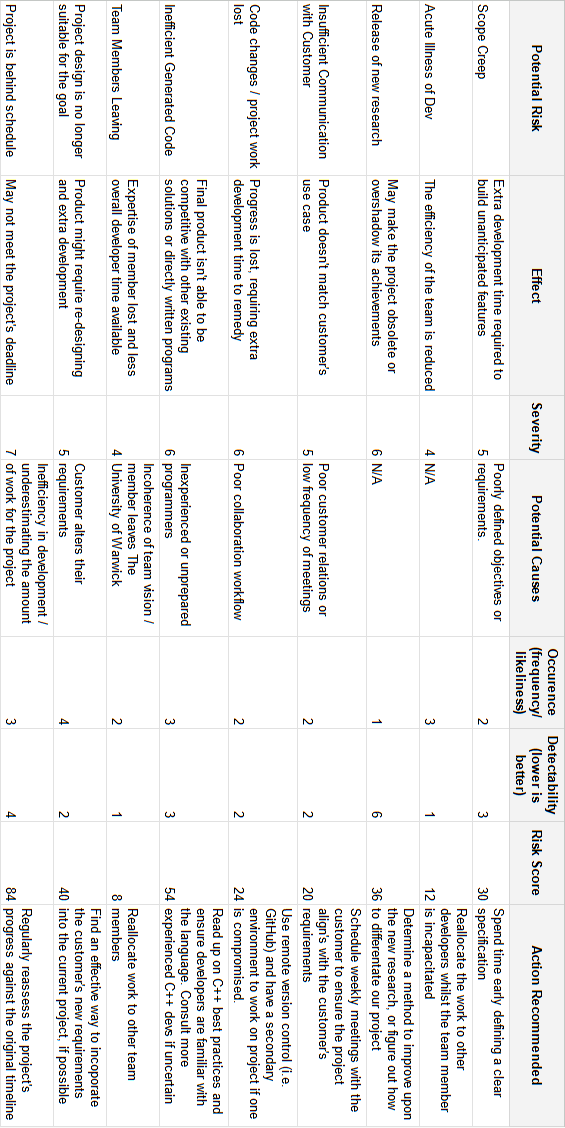
\includegraphics[width=10cm]{thesis/diagrams/risks.png}
    \caption{Failure Modes and Effects Analysis}
    \label{tab:fmea}
\end{table}


% TODO: Write this, also stakeholder analysis?
%\chapter{Business Case}
%The project's viability, and effects or benefits need to be considered in order to justify spending a large amount of time implementing it. This section discusses why this project is being undertaken, and who would potentially use such a product.

%\section{Domain-Specific Languages}

%\section{Scientists and Developers}

% TODO: proofing
\chapter{Legal, Social and Ethical Issues}

We have considered the legal, social and ethical implications of our project. We concluded that there are no immediate issues of concern in the specification of this project. However, as the project develops, we must be mindful and considerate of several factors. 

% Firstly: use of third party/open source libraries
Firstly, we will depend on a number of open source projects and libraries to develop the project; including but not limited to the miniapps for testing and verification, as well as the libraries to enable technologies to support various specialised hardware backends or other performance enhancing optimisations such as vectorisation. We must be careful to follow the licence terms of those projects and make it abundantly clear which sections of code were not written by ourselves. 

% Secondly: use of the DSL for bad thing?
Secondly, it is possible that the development of such a DSL could be used for projects and simulations which have unintended ethical consequences. Smoothed Particle Hydrodynamic simulations are used as tools in a large variety of industries, including complex particle interactions, nuclear engineering, and aeronautics. It is easy to imagine these fields may be used by, for example, military organisations. Hence, it is important to consider the moral implications of being associated with, or contributing to such fields.

% Thirdly: Environmental impact of HPC systems?
Finally, we should also consider the environmental impact of running these simulations. Our project is designed to be used for long-running, highly computationally intensive scientific simulations of complex physical phenomena. It is highly unlikely that these codes will be run on normal ``consumer grade'' hardware, but instead on high performance compute clusters. While in some regards, the use of centralised hardware which is shared between many different computing projects at any one time cuts down on extraneous electrical waste, power consumption, and by extension environmental impact; on the other hand, we must be mindful that long-running inefficient programs would cause a more adverse environmental impact in terms of radiated heat and power consumption and as such we should ensure that our project produces as efficient code as possible.

% TODO: Further Work section (needed?)

\glsaddall

\printbibliography[title={References}]

\end{document}
